% !TeX program = pdflatex
\documentclass[10pt,letterpaper,twocolumn]{article}

\usepackage[T1]{fontenc}
\usepackage{mathptmx,courier}
\usepackage{microtype}
\usepackage[letterpaper,top=0.71in,bottom=0.71in,left=0.74in,right=0.74in]{geometry}
\usepackage{graphicx}
\usepackage{booktabs}
\usepackage{array}
\usepackage[font=small,labelfont=bf]{caption}
\usepackage{dblfloatfix}
\usepackage{flushend}
\usepackage[hidelinks]{hyperref}

\setlength{\columnsep}{0.24in}
\setlength{\parindent}{1em}
\setlength{\parskip}{0pt}
\setlength{\textfloatsep}{12pt plus 3pt minus 2pt}
\setlength{\dbltextfloatsep}{12pt plus 3pt minus 2pt}
\setlength{\floatsep}{9pt plus 2pt minus 1pt}
\setlength{\dblfloatsep}{9pt plus 2pt minus 1pt}
\renewcommand{\dbltopfraction}{0.88}
\renewcommand{\topfraction}{0.86}
\renewcommand{\bottomfraction}{0.65}
\renewcommand{\textfraction}{0.10}
\renewcommand{\floatpagefraction}{0.77}
\renewcommand{\dblfloatpagefraction}{0.77}
\setcounter{topnumber}{3}
\setcounter{dbltopnumber}{3}
\setcounter{totalnumber}{5}
\captionsetup[figure]{skip=5pt}
\captionsetup[table]{position=top,skip=4pt}
\emergencystretch=0.9em
\raggedbottom

\hypersetup{
  pdftitle={KarBench: Can Language Models Calculate and Cite Indian Income Tax?},
  pdfauthor={Devraj Jhala},
  pdfsubject={Evaluation of tax calculation and statutory citation},
  pdfkeywords={Indian income tax, statutory citation, temporal legal reasoning, language model evaluation}
}

\title{\bfseries KarBench: Can Language Models Calculate and Cite\\ Indian Income Tax?}
\author{Devraj Jhala\\[2pt]
  \small Software Engineer}
\date{\small Revision 1.1, 24 November 2026}

\begin{document}

\twocolumn[{

  \maketitle

  \begin{center}

    \begin{minipage}{0.935\textwidth}

      \small

      \begin{center}\textbf{Abstract}\end{center}

      A language model can compute the right tax and still cite the wrong law. KarBench uses India's transition from the Income-tax Act, 1961 to the Income-tax Act, 2025 to measure these outcomes separately. We evaluate four model families from four providers in six configurations on the same 100 synthetic salaried profiles, crossed with three periods and three modes of access to rules (5,400 attempts). In closed-book Tax Year (TY) 2026--27, 303 of 600 attempts matched both rounded liabilities and the benchmark-designated regime, and zero supplied a complete citation set. With dated rules in context, 569 of 600 attempts supplied complete citations. Numeric scores measure agreement with an engine-generated reference under the recorded provider settings. Deadlines and cutoff enforcement differ by provider. A separate Grok-only analysis examines usable responses beyond the scoring cutoff.

      \par\medskip

      \noindent\textbf{Keywords:} Indian income tax \textperiodcentered{} statutory citation \textperiodcentered{} temporal legal reasoning \textperiodcentered{} language model evaluation

    \end{minipage}

  \end{center}

  \vspace{0.9em}

}]

\section{Introduction}

When an individual asks a language model how much income tax is due, the numeric result answers only part of the question. A reviewer also needs to establish which law governed the income period and which provisions support the calculation. Citations make it possible to distinguish a valid interpretation from an answer that reached the same amount by coincidence. A benchmark that grades only the amount can miss this distinction whenever two versions of the law yield the same liability.

India's recent statutory transition provides a concrete test. Assessment Year (AY) 2026--27 ordinarily refers to income earned in Financial Year (FY) 2025--26 under the Income-tax Act, 1961. Tax Year (TY) 2026--27 under the Income-tax Act, 2025 covers the following income period, beginning on 1 April 2026 \cite{act2025,taxfaq,pib}. Both labels contain ``2026--27,'' but the Act and key section numbers differ. For example, the rebate provision mapped by the benchmark changes from section 87A to section 156, and the new-regime provision changes from section 115BAC to section 202. A model can recognize the latest Act, reproduce the correct tax, and still supply a section from the earlier law or leave the field blank.

The difficulty is measurable in the reference data. For 98 of our 100 profiles, both final liabilities are identical under the two newest periods, even though the expected citations change. For all 100, the new-regime liability alone is identical across those periods. This overlap limits what we can infer from correct tax totals. It also gives us a paired design for asking whether models carry the correct legal authority through the calculation while holding the taxpayer's facts fixed.

KarBench evaluates three questions. \textbf{Can a model calculate and substantiate the tax from memory?} Closed-book answers let us observe exact tax, period selection and section-level citation on the same attempt. \textbf{How much does access to the applicable law change performance?} We compare directly supplied dated rules with an agent that must select and read evidence from an archive, then finish within a fixed budget. \textbf{How do inference limits change the result we measure?} We audit whether an output-limit label corresponds to missing answer text or a usable answer outside the benchmark ceiling, then report both the protocol result and an offline sensitivity analysis.

The study observes six model--provider configurations on 900 planned attempts each. Its contributions are 300 paired period-specific cases with deterministic reference traces, a citation rubric that distinguishes stale identifiers from required and inapplicable blanks, and an analysis of completion and cutoff behavior under the settings exercised here. The supplement documents the protocol and provides aggregate tables.

\section{Related work}

\textbf{Indian income tax.}
The LE-BTL study uses an IRAC+ rubric to evaluate legal reasoning on Indian tax questions, including income tax and GST \cite{lebtl}. The \texttt{itact-785} benchmark is the closest overlap on the 2025 Act. Its 785 locked tasks cover which Act applies across 1 April 2026, section crosswalks, tax deducted at source, and entity-level rates and deadlines. It uses strict entity matching without an LLM judge \cite{itact}. KarBench pairs identical salaried profiles across tax periods and scores two computed liabilities, regime choice, and statutory identifiers on each answer. It also varies access to dated rules within the same set of cases. Veeramani et al. compare an LLM-only system, retrieval, and a neuro-symbolic engine on 20 Indian tax scenarios under the 1961 Act \cite{ntol}.

\textbf{Temporal applicability and citation drift.}
\texttt{sanhita} tests section mapping and citation carry-over after India's IPC-to-BNS transition, including selecting the applicable criminal code for dated events \cite{sanhita}. Prior et al. use 312 expert-validated German statutory questions to study outdated responses after amendments and the use of current law for historical questions \cite{oldfriend}. Huang et al.'s TALD-Bench evaluates selection of the applicable statute version across China's civil-law transition \cite{tald}. LexKairos evaluates statutory temporal knowledge and case-based temporal reasoning in Chinese law \cite{lexkairos}. KarBench studies the same temporal failure modes in personal income tax. Its paired numerical keys let us test whether an incorrect liability matches another period and whether a correct liability can distinguish between periods.

\textbf{Tax computation and legal benchmarks.}
SARA pairs U.S. tax statutes with entailment and numerical questions \cite{sara}; TaxCalcBench measures U.S. personal tax calculation from taxpayer inputs \cite{taxcalcbench}. LegalBench and IL-TUR cover broader legal reasoning and Indian legal text understanding, respectively \cite{legalbench,iltur}. Related studies have examined the use of legal authority in Indian legal questions and errors about authorities in U.S. law \cite{courtready,legalfictions}. KarBench records obsolete identifiers, required blanks, and permitted rebate blanks separately.

\section{Benchmark and protocol}

\subsection{Case construction and dated authorities}

The development set comprises 100 synthetic resident salaried adults under 60. The first 20 profiles are diagnostic anchors, 40 emphasize thresholds, and 40 cover general cases. Every profile is instantiated in FY 2024--25, FY 2025--26 and TY 2026--27, for 300 cases. The task expresses the income period as a date range, year end, or FY/AY label in 102, 99 and 99 cases, respectively. The 60-case pilot is a subset of the same design.

Cases cover slabs, rebates and marginal relief, standard deduction, house rent allowance, retirement contributions, eligible savings interest, home-loan interest, health and education cess, and rounding. The scope excludes surcharge, special-rate income, business income and most investment income. Rule cards pin the period-specific provisions (Table~\ref{tab:authorities}). The 2026 rules also expand from four to eight the cities eligible for the 50\% salary term used in the house rent allowance formula \cite{rules2026}.

\begin{table}[!tb]
  \centering\small
  \setlength{\tabcolsep}{3pt}
  \caption{Period labels and statutory identifiers used in scoring. The 2025 Act standard deduction is in section 19(1). The benchmark pins accepted aliases by period \cite{act2025,taxfaq,pib,rules2026}.}
  \label{tab:authorities}
  \begin{tabular*}{\columnwidth}{@{\extracolsep{\fill}}lrrr@{}}
    \toprule
    \textbf{Field} & \textbf{FY 2024--25} & \textbf{FY 2025--26} & \textbf{TY 2026--27} \\
    \midrule
    Required label & AY 2025--26 & AY 2026--27 & TY 2026--27 \\
    Act & 1961 & 1961 & 2025 \\
    New regime & 115BAC & 115BAC & 202 \\
    Rebate section & 87A & 87A & 156 \\
    Std. deduction & 16(ia) & 16(ia) & 19 \\
    Rounding & 288A and 288B & 288A and 288B & 516 \\
    \bottomrule
  \end{tabular*}
\end{table}

A deterministic decimal-arithmetic engine computes both regimes and saves component and counterfactual traces. For each regime it discards paise and rounds total taxable income to the nearest INR\,10 before applying slabs. After rebate or marginal relief and cess, it again discards paise and rounds the final liability to the nearest INR\,10. A last digit of five rounds up at both stages (sections 288A and 288B of the 1961 Act and section 516 of the 2025 Act) \cite{round288a,round288b,act2025}. The new regime is designated on ties. In the two transition periods the new regime is strictly cheaper on 87/100 and 86/100 profiles, respectively. The old regime is cheaper on one case in each period. The other 12 and 13 are ties, which bring the designated new-regime share to 99/100 in each period.

\begin{table}[!tb]
  \centering\small
  \setlength{\tabcolsep}{3pt}
  \caption{Reference answer for the same INR\,12,75,000 salary profile (P0001) under three periods. The last two rows illustrate identical amounts under different statutory identifiers.}
  \label{tab:worked-example}
  \begin{tabular*}{\columnwidth}{@{\extracolsep{\fill}}lrrr@{}}
    \toprule
    \textbf{Period} & \textbf{Old tax} & \textbf{New tax} & \textbf{Rebate sec.} \\
    \midrule
    FY 2024--25 & INR\,1,87,200 & INR\,83,200 & 87A \\
    FY 2025--26 & INR\,1,87,200 & INR\,0 & 87A \\
    TY 2026--27 & INR\,1,87,200 & INR\,0 & 156 \\
    \bottomrule
  \end{tabular*}
\end{table}

The salary anchor in Table~\ref{tab:worked-example} illustrates the transition. FY 2025--26 and TY 2026--27 share the same zero new-regime liability after a INR\,60,000 rebate. An answer for the newer period that cites section 87A therefore satisfies the arithmetic on this case while failing the rebate citation field.

\subsection{Modes, model settings and stopping rules}

Each model receives a synthetic profile and a common output schema. \textbf{Closed book} offers no retrieval. \textbf{Rules in context} supplies the dated rule card. \textbf{Agent} offers archive search, archive reads and a calculator. The agent selects rules across the three-period archive and uses the provided arithmetic interface. General-purpose code execution is outside this tool interface. The materials omit scored-case reference answers.

\begin{table}[!tb]
  \centering\small
  \setlength{\tabcolsep}{3pt}
  \caption{Four providers and six model configurations. Each configuration evaluates exactly 900 planned case-mode pairs.}
  \label{tab:model-configurations}
  \begin{tabular*}{\columnwidth}{@{\extracolsep{\fill}}lllr@{}}
    \toprule
    \textbf{Provider} & \textbf{Endpoint} & \textbf{Reasoning} & \textbf{Attempts} \\
    \midrule
    DeepSeek & deepseek-flash & Thinking, low & 900 \\
    OpenAI & gpt-6-luna & Low, medium & 900 each \\
    Anthropic & claude-haiku-5-5 & Adaptive low, med. & 900 each \\
    xAI & grok-4.7 & Medium & 900 \\
    \bottomrule
  \end{tabular*}
\end{table}

The scoring limits are 8,192 metered output tokens per request and 16,384 per agent episode, with up to six agent turns and four tool calls per turn. The client request timeout was 240 seconds for DeepSeek, Luna and Haiku and 900 seconds for Grok. The first three use request-level output controls. For Grok the adapter checks output tokens after the response arrives and excludes over-cap rows from primary scores. Effective inference limits and reasoning presets are provider-specific. The frozen DeepSeek run records DeepSeek-V4.1-Flash-1017 as its expected model version. The primary results characterize each recorded model--provider configuration, including its adapter and timeout.

Each configuration contributes 300 attempts per mode and 100 in each mode-by-period cell. Recorded infrastructure retries preserve the intended case identity. DeepSeek replaced five infrastructure failures, one in closed book and four in agent mode. Haiku medium replaced three transport failures. The comparison retains one reviewed Luna medium transport failure, on a TY 2026--27 closed-book case. The protocol denominator remains 100 in that cell. Removing the failed row raises the exact-tax fraction from 62/100 to 62/99 and leaves the citation count at zero.

\subsection{Scoring, denominators and uncertainty}

\textbf{Exact tax} requires exact agreement with both rounded engine liabilities and the benchmark-designated regime. \textbf{Complete citations} requires the Act, period label and applicable section identifiers. \textbf{INR\,1 full answer} additionally tests intermediate fields with a tolerance of up to INR\,1 per field. The supplement reports \textbf{exact full answer} as a diagnostic that also requires exact intermediate traces. The diagnostic measures agreement with the benchmark's arithmetic convention for intermediate fields.

The shared comparison scorer accepts a blank rebate field when both reference and predicted rebate or relief are zero in both regimes. Elsewhere, blank required fields fail. Recognized prior-law identifiers and AY terminology under the 2025 Act are counted as stale. The remaining mismatches include unsupported identifiers and period-label strings outside the frozen accepted forms. The prompt explicitly asks models to leave unknown legal identifiers blank. A required blank is a failure to supply the reference under this setup.

Primary rates use every planned attempt and require a completed episode. Conditional rates use completed responses as the denominator. Our offline sensitivity analysis also scores parseable final JSON saved on output-limit rows and adds these passes to a separate numerator with the planned denominator. The original run status is retained. The 95\% intervals used for the rules-in-context gain are paired percentile intervals from 10,000 resamples of the 100 profiles, retaining all three years of each resampled profile. They characterize profile-set variation under this one-run design.

\section{Results}

\subsection{Tax accuracy improves when the dated rules are supplied}

Rules in context produced the highest exact-tax and INR\,1 full-answer rate in every configuration (Figure~\ref{fig:modes}). Across the three periods, DeepSeek's exact-tax success rose from 227/300 (75.7\%) in closed book to 288/300 (96.0\%) with rules, a 20.3 percentage-point gain (95\% profile interval 15.3--25.7). The smallest protocol-level gain was 18.0 points for Luna low (11.0--24.7). Grok's 49.3-point gain (43.3--55.3) partly reflects its much higher finish rate when rules were supplied. When its over-cap answers are included, the exact-tax gain is 4.7 points (280/300 to 294/300).

\begin{figure*}[!tb]
  \centering
  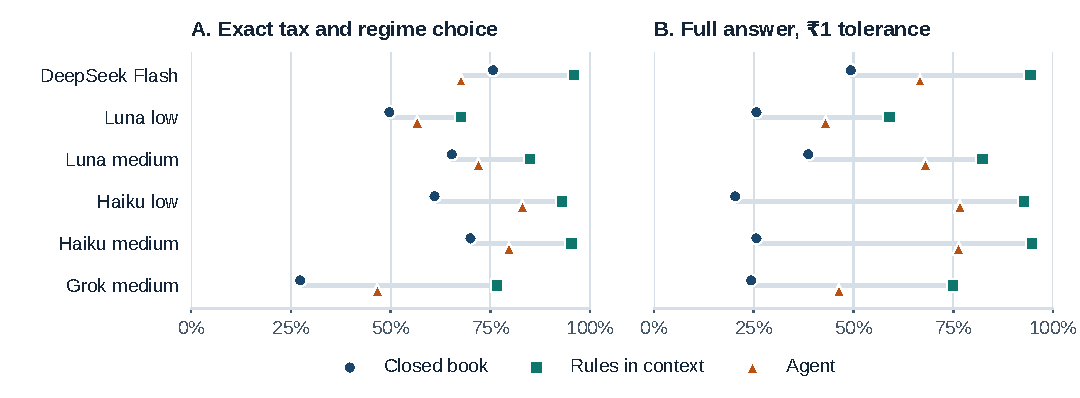
\includegraphics[width=0.92\textwidth]{figures/modes.pdf}
  \caption{Access-mode comparison across the six configurations. Each marker represents 300 planned attempts. Both panels use the full 0--100\% scale. Rule cards improve both metrics in every configuration relative to closed book.}
  \label{fig:modes}
\end{figure*}

\begin{table*}[!tb]
  \centering\small
  \setlength{\tabcolsep}{5pt}
  \caption{Scores under the recorded provider settings, 900 planned attempts per row. Exact tax includes regime choice. Complete citations can pass independently of tax.}
  \label{tab:all-scores}
  \begin{tabular*}{\textwidth}{@{\extracolsep{\fill}}lrrrr@{}}
    \toprule
    \textbf{Configuration} & \textbf{Finished} & \textbf{Exact tax} & \textbf{Complete citations} & \textbf{INR\,1 full answer} \\
    \midrule
    DeepSeek Flash & 737 (81.9\%) & 718 (79.8\%) & 649 (72.1\%) & 631 (70.1\%) \\
    Luna low & 829 (92.1\%) & 522 (58.0\%) & 709 (78.8\%) & 383 (42.6\%) \\
    Luna medium & 839 (93.2\%) & 667 (74.1\%) & 730 (81.1\%) & 567 (63.0\%) \\
    Haiku low & 898 (99.8\%) & 711 (79.0\%) & 714 (79.3\%) & 569 (63.2\%) \\
    Haiku medium & 868 (96.4\%) & 735 (81.7\%) & 704 (78.2\%) & 590 (65.6\%) \\
    Grok medium & 463 (51.4\%) & 452 (50.2\%) & 453 (50.3\%) & 437 (48.6\%) \\
    \bottomrule
  \end{tabular*}
\end{table*}

In rules in context, Haiku low and medium passed the INR\,1 full-answer score on 278/300 and 284/300 attempts, respectively. The exact intermediate-trace diagnostic gave 138/300 and 135/300. Across all Haiku-low modes, cess was the sole intermediate numeric mismatch on 214 of 377 exact-tax successes that failed exact full scoring. A row could also have a citation error. Exact full-answer scores remain in the supplement alongside final-liability and tolerance-based scores.

\subsection{Closed-book tax and citations diverge under the 2025 Act}

In TY 2026--27, 303/600 closed-book attempts passed exact tax within protocol (Table~\ref{tab:transition}). Zero supplied all the required citations. Every configuration had cases in which the tax and recommendation were correct but the legal references were incomplete. Complete citations were restored on 569/600 rule-assisted attempts and 480/600 agent attempts. All 569 finished rule-assisted responses had complete citations. In agent mode 480 of 482 finished answers had complete citations, with the other 118 attempts ending early.

\begin{table*}[!tb]
  \centering\small
  \setlength{\tabcolsep}{5pt}
  \caption{TY 2026--27 under the recorded settings, 100 planned attempts per configuration and mode. CB denotes closed book. Tax and citation counts include only in-protocol passes.}
  \label{tab:transition}
  \begin{tabular*}{\textwidth}{@{\extracolsep{\fill}}lrrrrr@{}}
    \toprule
    \textbf{Configuration} & \textbf{CB finished} & \textbf{CB exact tax} & \textbf{CB citations} & \textbf{Rules citations} & \textbf{Agent citations} \\
    \midrule
    DeepSeek Flash & 54 & 51 & 0 & 96 & 70 \\
    Luna low & 100 & 50 & 0 & 94 & 89 \\
    Luna medium & 99 & 62 & 0 & 95 & 88 \\
    Haiku low & 100 & 61 & 0 & 100 & 99 \\
    Haiku medium & 100 & 71 & 0 & 100 & 97 \\
    Grok medium & 9 & 8 & 0 & 84 & 37 \\
    \bottomrule
  \end{tabular*}
\end{table*}

Figure~\ref{fig:citations} shows how the field-level errors differ across models. DeepSeek named the old Act on 43/54 usable answers. Haiku low and medium named the correct Act on 100 and 99 of 100, respectively, but used a stale period label on 91 answers each. Luna medium supplied the correct new-regime section on 78/99. It omitted the rounding reference on 96 and gave a mismatching value on three. Across all six configurations, not a single closed-book answer in this period supplied a correct rounding reference.

A separate Grok-only analysis includes 91 usable closed-book TY 2026--27 answers that exceeded the scoring limit. Exact tax passed on 8 of 9 in-protocol and 80 of 91 over-cap responses (88/100 combined). All 100 identified the Act and period and left the section fields blank. Among the rebate blanks, 63 were inapplicable and 37 omitted an applicable identifier. The prompt allowed abstention on unknown identifiers.

\begin{figure*}[!tb]
  \centering
  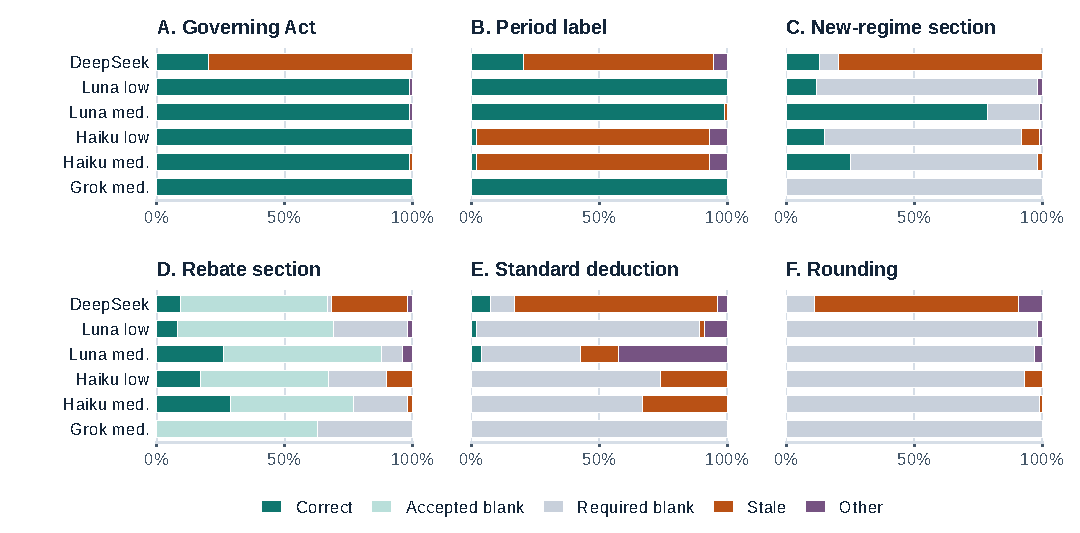
\includegraphics[width=0.97\textwidth]{figures/citations.pdf}
  \caption{Field-level decisions for usable closed-book TY 2026--27 responses. Sample sizes in model order are 54, 100, 99, 100, 100 and 100. Grok's bars include 91 parseable over-cap responses. An accepted blank is an inapplicable rebate field.}
  \label{fig:citations}
\end{figure*}

\subsection{Counterfactual-year tax signatures}

For every finished closed-book episode, the diagnostic compares the pair of reported rounded liabilities against all three reference periods for the same profile. The diagnostic uses the liability pair alone and excludes regime choice and citation fields. A pair equal to the intended year's key and an alternative year's key cannot identify which rules produced the answer.

Across 1,522 finished closed-book episodes, 270 pairs matched only the requested period, 777 matched it and at least one alternative, 12 matched an alternative while missing the requested period, and 463 matched none. Among the 475 episodes whose pair missed the requested period, 12 (2.5\%) matched an alternative. The corresponding counts were 1 for DeepSeek, 3 and 2 for Luna low and medium, 2 and 4 for Haiku low and medium, and 0 for Grok. This analysis uses the frozen run aggregates in Supplement Table B6 \cite{karbench}.

The two 1961 Act keys for FY 2024--25 and FY 2025--26 share both liabilities for 18 of the 100 profiles. A directional test would separately count mismatched FY 2025--26 responses that match FY 2024--25 and mismatched FY 2024--25 responses that match FY 2025--26. Table B6 pools target periods, so it does not resolve those counts. An alternative match is a signature of the tax amounts and cannot by itself identify which statute the model applied.

\subsection{Provider cutoffs and the Grok-only sensitivity analysis}

Grok's full run includes 463 completed episodes, 280 output-limit episodes, 122 tool-call-limit episodes and 35 turn-limit episodes. Completion in closed book declined from 46/100 in FY 2024--25 to 29/100 in FY 2025--26 and 9/100 in TY 2026--27. Rules in context finished 76, 76 and 84, respectively. The agent finished 49, 57 and 37, and its early endings came entirely from tool-call and turn ceilings. As Figure~\ref{fig:coverage} shows, the 463 completed episodes give different weights to the nine experimental cells. The conditional exact-tax rate of 452/463 (97.6\%) describes that selected subset (Table~\ref{tab:grok-conditional}).

\begin{figure*}[!tb]
  \centering
  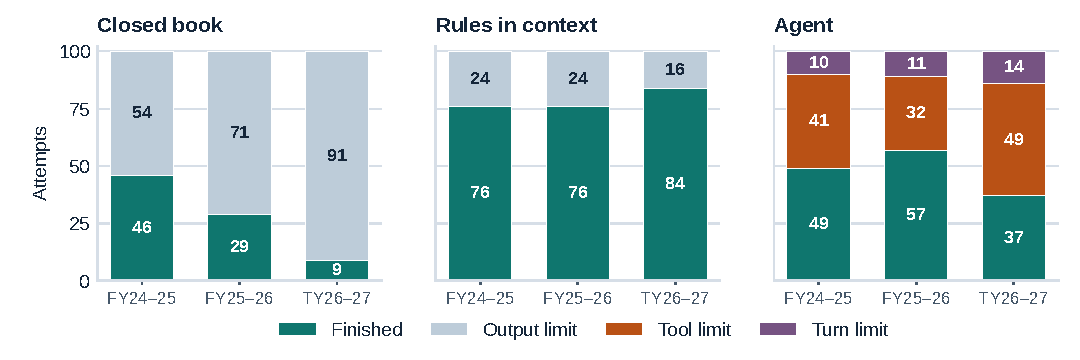
\includegraphics[width=0.92\textwidth]{figures/coverage.pdf}
  \caption{Grok run outcomes by mode and period. Each bar contains 100 attempts. The nine finished closed-book answers in TY 2026--27 represent 9\% of the cell, versus 46\% in the earliest period.}
  \label{fig:coverage}
\end{figure*}

\begin{table*}[!tb]
  \centering\small
  \setlength{\tabcolsep}{4pt}
  \caption{Grok performance on completed responses. Coverage uses all planned attempts. For the four score columns, $n$ is the number of passing answers and the percentage uses completed responses as its denominator.}
  \label{tab:grok-conditional}
  \begin{tabular*}{\textwidth}{@{\extracolsep{\fill}}llrrrrrrrr@{}}
    \toprule
    & \multicolumn{1}{c}{\textbf{Coverage}} &
      \multicolumn{2}{c}{\textbf{Exact tax}} &
      \multicolumn{2}{c}{\textbf{Complete citations}} &
      \multicolumn{2}{c}{\textbf{INR 1 full answer}} &
      \multicolumn{2}{c}{\textbf{Exact full answer}} \\
    \cmidrule(lr){2-2}\cmidrule(lr){3-4}\cmidrule(lr){5-6}\cmidrule(lr){7-8}\cmidrule(lr){9-10}
    \textbf{Mode} & \textbf{Finished / planned} & $n$ & \% & $n$ & \% & $n$ & \% & $n$ & \% \\
    \midrule
    Closed book & 84/300 & 82 & 97.6 & 74 & 88.1 & 73 & 86.9 & 68 & 81.0 \\
    Rules in context & 236/300 & 230 & 97.5 & 236 & 100.0 & 225 & 95.3 & 212 & 89.8 \\
    Agent & 143/300 & 140 & 97.9 & 143 & 100.0 & 139 & 97.2 & 138 & 96.5 \\
    \midrule
    All modes & 463/900 & 452 & 97.6 & 453 & 97.8 & 437 & 94.4 & 418 & 90.3 \\
    \bottomrule
  \end{tabular*}
\end{table*}

All 280 Grok output-limit episodes had provider status \texttt{completed} and parseable final JSON, with recorded output above 8,192 tokens. Their reported reasoning consumed 3,191,275 of 3,236,563 output tokens (98.6\%). Reasoning alone exceeded the limit on 270 rows. Reported output minus reported reasoning is a proxy for other output, including visible answer text. Its median on the capped Grok rows was 165 tokens, with a range of 142--175 (Figure~\ref{fig:tokens}). In the newest closed-book cell, median reasoning was 11,976 tokens, median other output was 150, and reasoning alone crossed the limit on 90/91 rows.

DeepSeek's 72 output-limit episodes instead ended with provider reason \texttt{length}. Seventy-one contained empty final text and one contained text that failed JSON parsing. Their total reported reasoning was 589,720 tokens, with only 104 other output tokens. Neither Luna nor Haiku had a recorded output-limit termination. These differences concern the observed provider and runner behavior. The benchmark applied the same nominal ceiling with different enforcement mechanisms.

\begin{figure*}[!tb]
  \centering
  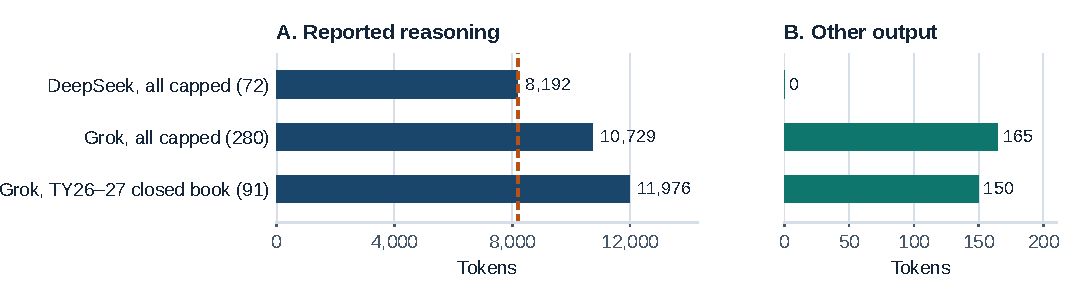
\includegraphics[width=0.92\textwidth]{figures/tokens.pdf}
  \caption{Median component counts on capped responses. Other output is total metered output minus reported reasoning. Axes differ by panel. The dashed line marks the benchmark's 8,192-token request ceiling.}
  \label{fig:tokens}
\end{figure*}

The Grok-only analysis adds 198 closed-book and 64 rule-assisted exact-tax successes across the three periods (Figure~\ref{fig:sensitivity}). Grok's primary score of 452/900 becomes 714/900 when its usable over-cap answers are included. In TY 2026--27 the closed-book citation count remains zero and the rule-assisted count rises from 84/100 to 100/100. These counts describe saved outputs beyond the scoring limit for one provider.

\begin{figure*}[!tb]
  \centering
  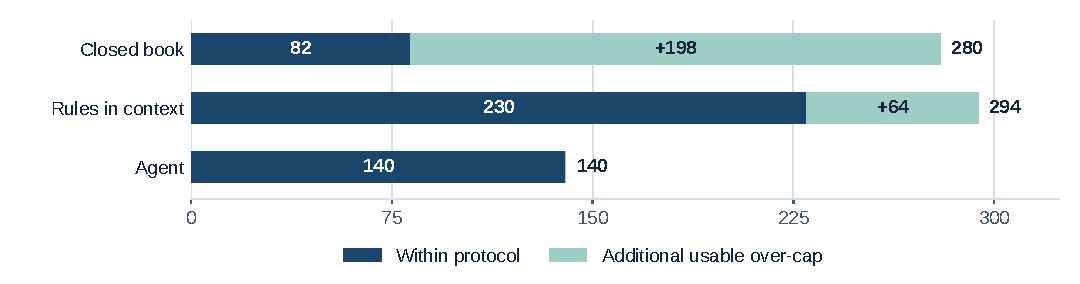
\includegraphics[width=0.90\textwidth]{figures/sensitivity.pdf}
  \caption{Grok exact-tax and regime-choice counts with usable over-cap answers added offline. Each mode has 300 planned attempts. The total at the end of each bar uses the same denominator as the protocol score.}
  \label{fig:sensitivity}
\end{figure*}

\subsection{Tool use, metering and cost}

Tool limits affected completed workflows as well as early endings (Table~\ref{tab:tool-use}). Of 209 successful DeepSeek agent episodes, 121 used the maximum four tools in at least one turn and 31 finished on turn six. The corresponding Grok values were 79 and 27 of 143. Successful agent episodes used a median of seven tools for DeepSeek and six for Grok, counted across turns. Tool-call-limit endings across configurations ranged from 2 for Haiku low to 122 for Grok. A direct rule card removes evidence selection and the additional calls required for retrieval, which helps explain why the agent comparisons should be interpreted as workflow outcomes.

\begin{table}[!tb]
  \centering\small
  \setlength{\tabcolsep}{3pt}
  \caption{Tool use on completed agent episodes. Done counts completed episodes. Tools is the total executions, Median is tools per episode, At 4 counts episodes reaching four in a turn, and Turn 6 counts completions on the sixth turn.}
  \label{tab:tool-use}
  \begin{tabular*}{\columnwidth}{@{\extracolsep{\fill}}lrrrrr@{}}
    \toprule
    \textbf{Configuration} & \textbf{Done} & \textbf{Tools} & \textbf{Median} & \textbf{At 4} & \textbf{Turn 6} \\
    \midrule
    DeepSeek Flash & 209 & 1549 & 7 & 121 & 31 \\
    Luna low & 266 & 1120 & 4 & 75 & 1 \\
    Luna medium & 251 & 1070 & 4 & 73 & 13 \\
    Haiku low & 298 & 935 & 3 & 3 & 0 \\
    Haiku medium & 268 & 1139 & 4 & 35 & 0 \\
    Grok medium & 143 & 999 & 6 & 79 & 27 \\
    \bottomrule
  \end{tabular*}
\end{table}

\begin{table}[!tb]
  \centering\small
  \setlength{\tabcolsep}{3pt}
  \caption{Local USD ledger for the full runs at saved precision. The reserve records unresolved requests. Ledger equals usage plus reserve; the Total row sums each column. These values are local estimates.}
  \label{tab:costs}
  \begin{tabular*}{\columnwidth}{@{\extracolsep{\fill}}lrrrr@{}}
    \toprule
    \textbf{Configuration} & \textbf{Usage} & \textbf{Reserve} & \textbf{Ledger} & \textbf{Cap} \\
    \midrule
    DeepSeek Flash & \$6.5085699 & \$0.0723672 & \$6.5809371 & \$10.00 \\
    Luna low & \$0.7589530 & \$0.0286758 & \$0.7876288 & \$10.00 \\
    Luna medium & \$1.0400283 & \$0.0115202 & \$1.0515485 & \$3.00 \\
    Haiku low & \$1.3319712 & \$0.0000000 & \$1.3319712 & \$4.00 \\
    Haiku medium & \$1.5274349 & \$0.0233070 & \$1.5507419 & \$4.00 \\
    Grok medium & \$44.0503040 & \$3.2596760 & \$47.3099800 & \$48.50 \\
    \midrule
    Total & \$55.2172613 & \$3.3955462 & \$58.6128075 & --- \\
    \bottomrule
  \end{tabular*}
\end{table}

Table~\ref{tab:costs} reports the saved precision so that rows and columns reconcile. The corresponding amounts rounded to cents are \$55.22 in recorded usage, \$3.40 in unresolved reservations, and \$58.61 for the combined ledger total. The aggregate is rounded after summing the saved values. Grok's recorded usage includes its 60-episode pilot once. Provider invoice amounts can differ from these local estimates.

A retrospective filter across the single-request modes retains only in-protocol completions with logged end-to-end episode time of at most 240 seconds. It leaves TY 2026--27 totals at 303/600 for closed-book exact tax, 0/600 for closed-book complete citations, and 569/600 for rule-assisted complete citations. Across all periods this filter removes two completed Grok rule-assisted episodes and one Luna-low rule-assisted episode (Supplement Table C5).

\section{Discussion and limitations}

\textbf{A correct amount is a weak test of current authority.} The paired profiles reveal why legal benchmarks need both numeric and source-level criteria. Most liabilities in the two latest periods are identical, so an answer can appear correct under either statute. Some models transfer older identifiers, others supply the new Act without the new period label, and Grok abstains on section fields. Scoring each field makes those differences visible. A legal workflow can use such signals to decide when to ask for supporting text or request human review.

\textbf{Comparability and missing answers.} The recorded deployment settings constrain the interpretation of cross-system scores. An API cutoff can leave less usable text than an offline output cutoff. Grok's usable over-cap answers contribute only to its provider-specific sensitivity analysis. Conditional accuracy depends on which episodes finish. A controlled comparison would require similarly enforced output caps, a matching request deadline, and comparable inference budgets.

\textbf{Scope and reference validation.}
The synthetic, English-language cases isolate tax-period and citation effects for structured resident salaried profiles. The 5,400 attempts reuse the same 100 profiles. Document extraction, capital gains and legal ambiguity fall outside the case design. The regime-label imbalance makes recommendation-only accuracy weak evidence. Broader workflow evaluation would need a less skewed case set, real-document tasks and a code-enabled baseline with the same evidence.

Recomputing the pinned engine reproduced the 300 reference answers. A separate script verifies both rounding stages in all 600 saved regime traces using the recorded components. It checks arithmetic consistency at those stages. A separate calculation of the salary anchor reproduced both liabilities in AY 2025--26 and AY 2026--27 \cite{salaried25,salaried26}. A chartered accountancy student provided qualitative feedback on a 30-case packet and identified the HRA wording issue. A case-by-case independent legal audit of the full reference remains outstanding. The reported exact scores measure agreement with the frozen engine key.

\textbf{HRA prompt wording.} The common prompt stated that rent was actually paid for accommodation the employee did not own. In 210 of the 300 cases (70 profiles), the structured inputs specify zero rent and zero HRA. In rent-paying cases, the clause clarifies the eligibility facts for the old-regime exemption. The engine uses the structured amounts and yields zero HRA exemption in both regimes for the 210 zero-input cases. The reported evaluation used the original wording. Its effect on model responses was not measured.

\textbf{Interpretation of omissions.} The instructions permit blanks when identifiers are unknown. Our closed-book finding concerns observed omissions and stale citations under this prompt. A citation-only test with a separate abstention condition could measure what models supply when they are asked directly for each provision. Neither conditional accuracy nor the cap sensitivity isolates provider, model family and reasoning preset effects.

\section{Conclusion}

KarBench separates agreement on tax calculations from citation completeness for the 2025 Act on a controlled synthetic benchmark. In the recorded configurations, 303/600 closed-book attempts matched the engine's two liabilities and designated regime, and zero supplied a complete citation set. Rule-assisted attempts supplied complete citations in 569/600 cases. The findings support reporting amounts, legal references, and coverage separately. Generalization to other profiles and controlled provider comparisons requires further evidence.

\section*{Data and code availability}

The \href{https://github.com/Devrajsinh-Jhala/KarBench}{public KarBench repository} \cite{karbench} hosts the supplement and aggregate CSVs, including scores by mode and period, citation buckets, protocol hashes, token counts, cost ledgers, and frozen run identifiers. The repository also hosts the frozen synthetic cases, reference answers, and authored rule cards. Full row-level reproduction requires the original provider outputs and matching experiment snapshots.

\section*{Acknowledgments and AI disclosure}

Anthropic Claude \cite{claude} suggested the initial benchmark idea and supported early project development. OpenAI ChatGPT \cite{chatgpt} assisted with manuscript drafting, revision and figure preparation based on the recorded benchmark results. The author is responsible for the reported methods and claims.


\begin{thebibliography}{99}

\small

\bibitem{act2025}
Government of India. \textit{Income-tax Act, 2025}, as amended by the Finance Act, 2026. Act 30 of 2025, §§ 1, 3, 19, 156, 202, 516, 536. \href{https://www.incometaxindia.gov.in/documents/d/guest/income\_tax\_act\_2025\_as\_amended\_by\_fa\_act\_2026-pdf}{Official text}

\bibitem{taxfaq}
Income Tax Department. \textit{General Questions FAQs}. Guidance on the transition from Assessment Year 2026--27 to Tax Year 2026--27. \href{https://www.incometax.gov.in/iec/foportal/help/all-topics/e-filing-services/General\%20Questions-faqs}{Department guidance}

\bibitem{pib}
Press Information Bureau, Ministry of Finance. \textit{Income-tax Act, 2025 comes into force from today (1st April, 2026)}. 1 April 2026. \href{https://www.pib.gov.in/PressReleasePage.aspx?PRID=2248005\&lang=1\&reg=3}{Release}

\bibitem{rules2026}
Central Board of Direct Taxes. \textit{Income-tax Rules, 2026}. Notification 22/2026, G.S.R. 198(E), 20 March 2026, Rule 279. \href{https://www.incometaxindia.gov.in/documents/d/guest/en-notified-it-rules-2026-20-03-2026-pdf}{Notified text}

\bibitem{lebtl}
N. Jain, N. Wadhwa, P. Goyal, S. Ghosh, S. Pawar, A. Shinde, K. Boinepally, V. V. Malpani, and R. K.
LLM evaluations for Bharat Tax Laws (LE-BTL). A framework to evaluate and benchmark the accuracy of large language models in the context of the Indian tax laws. SSRN 5941734, 2025.
\href{https://www.taxmann.com/post/blog/taxmann-ai-x-iit-kharagpur-llm-evaluation-le-btl-benchmark-study}{Study overview}.

\bibitem{itact}
Prasthana Lab. \emph{itact-785: Evaluation of applied Indian tax-law compliance under the Income-tax Act, 2025}. Repository and benchmark, 2026.
\href{https://github.com/bugyal/itact-785/blob/30f97fdd2adc1b4c301832bd4116c642cd856eca/README.md}{Pinned repository documentation}.

\bibitem{ntol}
K. Veeramani, Allen Joseph N, and Pavithran M.
Neuro-symbolic reasoning engine for tax optimisation. \emph{Frontiers in Artificial Intelligence}, 9:1802755, 2026.
\href{https://doi.org/10.3389/frai.2026.1802755}{doi:10.3389/frai.2026.1802755}.

\bibitem{sanhita}
rishikeshn-eng. \emph{sanhita}. Indian criminal-code citation checker and benchmark.
\href{https://github.com/rishikeshn-eng/sanhita}{Source repository}.

\bibitem{oldfriend}
M. Prior, A. Schultz, and M. Grabmair.
Asking for an old friend: Diagnosing and mitigating temporal failure modes in LLM-based statutory question answering. 2026.
\href{https://arxiv.org/abs/2605.23497}{arXiv:2605.23497}.

\bibitem{tald}
Y. Huang et al.
When do LLMs apply the wrong law? Diagnosing LLM failures in temporal legal reasoning. 2026.
\href{https://arxiv.org/abs/2608.14610}{arXiv:2608.14610}.

\bibitem{sara}
Holzenberger, N., Blair-Stanek, A., and Van Durme, B. A dataset for statutory reasoning in tax law entailment and question answering. \textit{Natural Legal Language Processing Workshop}, 2020. \href{https://arxiv.org/abs/2005.05257}{arXiv:2005.05257}

\bibitem{taxcalcbench}
Bock, M. R., Molisee, K., Ozer, Z., and Shah, S. TaxCalcBench: Evaluating frontier models on the tax calculation task. 2025. \href{https://arxiv.org/abs/2507.16126}{arXiv:2507.16126}

\bibitem{legalbench}
Guha, N., et al. LegalBench: A collaboratively built benchmark for measuring legal reasoning in large language models. \textit{NeurIPS Datasets and Benchmarks}, 2023. \href{https://proceedings.neurips.cc/paper\_files/paper/2023/hash/89e44582fd28ddfea1ea4dcb0ebbf4b0-Abstract-Datasets\_and\_Benchmarks.html}{Proceedings}

\bibitem{iltur}
Joshi, A., Paul, S., Sharma, A., Goyal, P., Ghosh, S., and Modi, A. IL-TUR: Benchmark for Indian Legal Text Understanding and Reasoning. \textit{Proceedings of the 62nd Annual Meeting of the Association for Computational Linguistics}, pp. 11460--11499, 2024. \href{https://aclanthology.org/2024.acl-long.618/}{ACL Anthology}

\bibitem{courtready}
Juvekar, K., Bhattacharya, A., Khadloya, S., and Saxena, U. Are LLMs court-ready? Evaluating frontier models on Indian legal reasoning. \textit{Natural Legal Language Processing Workshop}, 2025. \href{https://aclanthology.org/2025.nllp-1.26/}{ACL Anthology}

\bibitem{legalfictions}
Dahl, M., Magesh, V., Suzgun, M., and Ho, D. E. Large legal fictions: Profiling legal hallucinations in large language models. \textit{Journal of Legal Analysis}, 16(1), 2024. \href{https://arxiv.org/abs/2401.01301}{arXiv:2401.01301}

\bibitem{karbench}
Jhala, D. \textit{KarBench}. Dataset, preprint, aggregate results, and supplementary methods, 2026. \href{https://github.com/Devrajsinh-Jhala/KarBench}{GitHub repository}

\bibitem{salaried25}
Income Tax Department. Salaried individuals for AY 2025--26. Tax slabs and guidance.
\href{https://www.incometax.gov.in/iec/foportal/help/individual/return-applicable-3}{Department guidance}.

\bibitem{salaried26}
Income Tax Department. Salaried individuals for AY 2026--27. Tax slabs and guidance.
\href{https://www.incometax.gov.in/iec/foportal/help/individual/return-applicable-1}{Department guidance}.

\bibitem{claude}
Anthropic. \textit{Claude}. Generative AI assistant. \href{https://www.anthropic.com/claude}{Product documentation}

\bibitem{chatgpt}
OpenAI. \textit{ChatGPT}. Generative AI assistant. \href{https://openai.com/chatgpt/overview/}{Product documentation}

\bibitem{lexkairos}
Li, C., Feng, Z., Huang, Y., Ye, Y., and Xie, H. LexKairos: Benchmarking Legal Temporal Capabilities in LLMs. 2026. \href{https://arxiv.org/abs/2608.09106}{arXiv:2608.09106}

\bibitem{round288a}
Government of India. Income-tax Act, 1961, section 288A. \href{https://www.incometaxindia.gov.in/w/section-288a-31}{Income Tax Department}

\bibitem{round288b}
Government of India. Income-tax Act, 1961, section 288B. \href{https://wm.incometaxindia.gov.in/w/section-288b-50}{Income Tax Department}

\end{thebibliography}

\end{document}
